\documentclass[journal]{IEEEtran}
\usepackage{amsmath,amsfonts}
\usepackage{algorithmic}
\usepackage{algorithm}
\usepackage{array}
\usepackage[caption=false,font=normalsize,labelfont=sf,textfont=sf]{subfig}
\usepackage{textcomp}
\usepackage{stfloats}
\usepackage{url}
\usepackage{verbatim}
\usepackage{graphicx}
\usepackage{cite}
\usepackage{float}
\hyphenation{op-tical net-works semi-conduc-tor IEEE-Xplore}
% updated with editorial comments 8/9/2021

\begin{document}

\title{Formulação dos Índices de Distribuição de Potência para Fluxos de Potência Lineares }

\author{Gabriel H. Limp,~\IEEEmembership{Aluno,~UFJF,}
        Giovani S. Junqueira,~\IEEEmembership{Aluno,~UFJF}%
        \thanks{Gabriel H. Limp e Giovani S. Junqueira são alunos da Faculdade de Engenharia El\'etrica, Universidade Federal de Juiz de Fora, MG. (e-mails: gabriel.halfeld@estudante.ufjf.br; giovani.junqueira@estudante.ufjf.br)}%
        \thanks{Manuscript recebido em Junho 2025; revisado em Julho 2025.}
}
        % <-this % stops a space
% \thanks{This paper was produced by the IEEE Publication Technology Group. They are in Piscataway, NJ.}% <-this % stops a space
% \thanks{Manuscript received April 19, 2021; revised August 16, 2021.}}

% The paper headers
\markboth{Trabalho proposto na Disciplina de Análise de Redes do PPEE da UFJF, Junho~2025}%
{Shell \MakeLowercase{\textit{et al.}}: A Sample Article Using IEEEtran.cls for IEEE Journals}

% \IEEEpubid{0000--0000/00\$00.00~\copyright~2021 IEEE}
% Remember, if you use this you must call \IEEEpubidadjcol in the second
% column for its text to clear the IEEEpubid mark.

\maketitle

\begin{abstract}
This study revisits and mathematically formalizes heuristic methods widely used to estimate power flows in electric networks through distribution factors. Based on the classical work by P. W. Sauer (1981), three main formulations are analyzed: (i) current distribution factors, (ii) distribution factors assuming constant voltage at the swing bus, and (iii) distribution factors with an arbitrary ground tie — the latter generalizing the former two. The paper demonstrates that these approaches, although initially empirical, are valid approximations of the exact solution under linear conditions. Independent simulations were conducted to verify the consistency among formulations and to assess the impact of different assumptions on the resulting power flows. Results confirm that distribution factors are an effective tool for contingency analysis, linear dispatch models, and fast operational assessments, providing sufficient accuracy with significant computational efficiency. 
\end{abstract}

\begin{IEEEkeywords}
Power Flow, Power Systems, Linear Load Flow. % REVISAR
\end{IEEEkeywords}

\section{Introdução}
\IEEEPARstart{O}{fluxo de carga} é uma das ferramentas mais fundamentais da análise de sistemas elétricos de potência, sendo utilizado em estudos de planejamento, operação e avaliação de contingências. Muitas dessas aplicações, principalmente aquelas que demandam processamento em tempo real ou múltiplas iterações, o uso de métodos rápidos e aproximados tem se mostrado altamente eficiente.

Entre os métodos rápidos amplamente utilizados, destacam-se aqueles baseados em fatores de distribuição de potência, que permitem estimar os fluxos de potência nas linhas a partir das potências injetadas nas barras, sem a necessidade de resolver iterativamente o sistema de equações completo. Esses fatores são particularmente úteis em aplicações como análise de contingências (\textit{N}-1), estudos de intercâmbio entre áreas, despacho econômico linearizado, fluxos ótimos simplificados e algoritmos de planejamento com redução do espaço de busca.

Apesar de sua ampla aplicação, a formulação desses fatores é frequentemente baseada em hipóteses heurísticas, como a utilização da barra swing como referência ou a introdução de ligações artificiais ao terra. Nesse contexto, o artigo clássico de P. W. Sauer, \textit{On the Formulation of Power Distribution Factors for Linear Load Flow Methods}, apresenta uma contribuição significativa ao estabelecer uma base matemática sólida para esses métodos.

O presente trabalho tem como objetivo revisar as três formulações propostas por Sauer: (i) os fatores de distribuição de corrente, (ii) os fatores com tensão constante na barra swing, e (iii) os fatores com ligação arbitrária ao terra — sendo este último uma generalização dos anteriores. São também realizadas simulações próprias para validar os conceitos, verificar a coerência entre os métodos e avaliar suas vantagens em termos de simplicidade computacional e precisão nas estimativas de fluxo.

\section{Formulação dos Fatores de Distribuição}

A formulação dos fatores de distribuição proposta em~\cite{ref1} busca representar, de forma linear, a relação entre as correntes ou potências que circulam nas linhas de transmissão e as injeções de corrente líquida nas barras do sistema. Essa abordagem é particularmente útil em análises rápidas de rede, permitindo estimar a resposta da malha elétrica a perturbações sem resolver iterativamente o fluxo de carga completo.

No chamado \textit{Caso A}, as correntes nas linhas são expressas diretamente em função das correntes injetadas nas barras por meio da seguinte relação matricial:

\begin{equation}
\begin{bmatrix}
I^{A}_{12} \\
I^{A}_{13} \\
\vdots \\
I^{A}_{ij} \\
\vdots \\
I^{A}_{mn}
\end{bmatrix}
=
\begin{bmatrix}
T_{12,1} & T_{12,2} & \cdots & T_{12,n} \\
T_{13,1} & T_{13,2} & \cdots & T_{13,n} \\
\vdots & \vdots & \ddots & \vdots \\
T_{ij,1} & T_{ij,2} & \cdots & T_{ij,n} \\
\vdots & \vdots & \ddots & \vdots \\
T_{mn,1} & T_{mn,2} & \cdots & T_{mn,n}
\end{bmatrix}
\cdot
\begin{bmatrix}
I^{A}_{1} \\
I^{A}_{2} \\
\vdots \\
I^{A}_{l} \\
\vdots \\
I^{A}_{n}
\end{bmatrix}
\label{eq:corrente_casoA}
\end{equation}

Considerando pequenas perturbações no sistema, pode-se linearizar a relação acima e representar apenas as variações incrementais de corrente. Surge então a forma:

\begin{equation}
\begin{bmatrix}
\Delta I_{12} \\
\Delta I_{13} \\
\vdots \\
\Delta I_{ij} \\
\vdots \\
\Delta I_{mn}
\end{bmatrix}
=
\begin{bmatrix}
T_{12,1} & T_{12,2} & \cdots & T_{12,n} \\
T_{13,1} & T_{13,2} & \cdots & T_{13,n} \\
\vdots & \vdots & \ddots & \vdots \\
T_{ij,1} & T_{ij,2} & \cdots & T_{ij,n} \\
\vdots & \vdots & \ddots & \vdots \\
T_{mn,1} & T_{mn,2} & \cdots & T_{mn,n}
\end{bmatrix}
\cdot
\begin{bmatrix}
\Delta I_{1} \\
\Delta I_{2} \\
\vdots \\
\Delta I_{l} \\
\vdots \\
\Delta I_{n}
\end{bmatrix}
\label{eq:corrente_incremental}
\end{equation}

Alternativamente, pode-se trabalhar diretamente com potências aparentes, caso em que os fatores de distribuição são aplicados sobre as variações de \( \Delta S_k \), e a matriz é conjugada. A expressão assume então a forma:

\begin{equation}
\begin{bmatrix}
\Delta S_{12} \\
\Delta S_{13} \\
\vdots \\
\Delta S_{ij} \\
\vdots \\
\Delta S_{mn}
\end{bmatrix}
=
\begin{bmatrix}
T^{*}_{12,1} & T^{*}_{12,2} & \cdots & T^{*}_{12,n} \\
T^{*}_{13,1} & T^{*}_{13,2} & \cdots & T^{*}_{13,n} \\
\vdots & \vdots & \ddots & \vdots \\
T^{*}_{ij,1} & T^{*}_{ij,2} & \cdots & T^{*}_{ij,n} \\
\vdots & \vdots & \ddots & \vdots \\
T^{*}_{mn,1} & T^{*}_{mn,2} & \cdots & T^{*}_{mn,n}
\end{bmatrix}
\cdot
\begin{bmatrix}
\Delta S_{1} \\
\Delta S_{2} \\
\vdots \\
\Delta S_{l} \\
\vdots \\
\Delta S_{n}
\end{bmatrix}
\label{eq:potencia}
\end{equation}

As diferentes formas de obtenção da matriz \( T \) dependem da escolha das condições de referência impostas ao sistema. No artigo, são propostas três estratégias distintas: (i) utilização direta da matriz de impedância reduzida, (ii) consideração de tensão constante na barra swing, e (iii) ligação arbitrária ao terra. Essas abordagens serão detalhadas nas subseções a seguir.

\subsection{Fatores de Distribuição de Corrente}

Nesta formulação, considera-se a matriz de impedância \( z \) obtida a partir do sistema com a barra de referência (ou swing) já eliminada. A ideia central é calcular a corrente na linha \( ij \), provocada por uma injeção de corrente unicamente na barra \( l \), utilizando a diferença entre as impedâncias de acoplamento das barras \( i \) e \( j \) com a barra \( l \), normalizada pela impedância total da linha.

A expressão resultante do fator de distribuição de corrente é dada por:

\begin{equation}
T_{ij,l} = \frac{z_{il} - z_{jl}}{\bar{z}_{ij}}
\label{eq:fdc}
\end{equation}

Nesta equação:
\begin{itemize}
  \item \( z_{il} \) e \( z_{jl} \) representam os elementos da matriz de impedância entre as barras \( i \) e \( j \) com a barra \( l \);
  \item \( \bar{z}_{ij} \) é a impedância da linha entre as barras \( i \) e \( j \), com conjugação complexa;
  \item \( T_{ij,l} \) representa o fator de distribuição de corrente da linha \( ij \) com relação à injeção na barra \( l \).
\end{itemize}

A matriz \( z \) utilizada é construída com a exclusão da barra de referência, e os fatores \( T_{ij,l} \) obtidos com essa formulação correspondem à distribuição de corrente no sistema quando a tensão da barra swing é livre para variar em resposta às perturbações. Esta abordagem corresponde ao que o artigo denomina de \textit{caso base não referenciado}, sendo considerada a forma mais elementar dos fatores de distribuição de corrente.

\subsection{Fatores com Tensão Constante na Barra Swing}

Nesta formulação, adota-se a premissa de que a tensão da barra swing permanece constante, tanto em módulo quanto em ângulo, frente a variações nas injeções de corrente líquida. Essa hipótese equivale a considerar que a barra de referência possui impedância infinita com o terra, o que impõe uma condição de tensão fixa no sistema.

Sob essa hipótese, os fatores de distribuição são ajustados de forma a considerar a influência da swing sobre a redistribuição de corrente nas linhas. O fator de distribuição modificado para a linha \( ij \) com relação à injeção na barra \( l \) é definido por:

\begin{equation}
T'_{ij,l} = \left( \frac{z_{il} - z_{jl}}{\bar{z}_{ij}} \right) - \frac{z_{1l}}{z_{11}} \cdot \left( \frac{z_{i1} - z_{j1}}{\bar{z}_{ij}} \right)
\label{eq:swing}
\end{equation}

Nessa equação:
\begin{itemize}
  \item \( z_{il} \) e \( z_{jl} \) correspondem às impedâncias entre as barras \( i \), \( j \) e a barra \( l \);
  \item \( z_{i1} \), \( z_{j1} \) e \( z_{1l} \) são os elementos da matriz de impedância entre as respectivas barras e a barra swing (denotada como barra 1);
  \item \( \bar{z}_{ij} \) representa o conjugado da impedância da linha entre \( i \) e \( j \);
  \item \( T'_{ij,l} \) é o fator de distribuição ajustado pela referência de tensão fixa na swing.
\end{itemize}

O termo subtraído na Equação~\eqref{eq:swing} representa a compensação causada pela imposição da tensão constante na barra swing. Esta compensação corrige a influência indireta da injeção em \( l \) sobre a tensão nas demais barras via a swing. Essa abordagem é comumente utilizada por sua simplicidade e aderência aos modelos clássicos de fluxo de carga com barra de referência fixa.

\subsection*{C. Fatores com Ligação Arbitrária ao Terra (1\,+\,j1)}

Nesta formulação, introduz-se uma ligação de impedância arbitrária entre a barra de referência e o terra, modelada como uma impedância finita \( z_{\text{tie}} \). Essa abordagem permite simular um caso intermediário entre os extremos de tensão constante (barra swing com impedância infinita) e de rede não referenciada (sem barra swing definida), generalizando os métodos anteriores.

A equação correspondente ao fator de distribuição de corrente da linha \( ij \) com relação à injeção na barra \( l \), considerando a impedância de amarração ao terra, é expressa por:

\begin{equation}
T^{\text{tie}}_{ij,l} = \left( \frac{z_{il} - z_{jl}}{\bar{z}_{ij}} \right) - \frac{z_{1l}}{z_{11} - \bar{z}_{\text{tie}}} \cdot \left( \frac{z_{i1} - z_{j1}}{\bar{z}_{ij}} \right)
\label{eq:lig_terra}
\end{equation}

Nessa equação:
\begin{itemize}
  \item \( z_{il} \), \( z_{jl} \), \( z_{i1} \), \( z_{j1} \) e \( z_{1l} \) são elementos da matriz de impedância entre as barras \( i \), \( j \), \( 1 \) (swing) e \( l \);
  \item \( \bar{z}_{ij} \) é a impedância da linha entre \( i \) e \( j \), com conjugado complexo;
  \item \( \bar{z}_{\text{tie}} \) representa a impedância equivalente da ligação ao terra;
  \item \( T^{\text{tie}}_{ij,l} \) é o fator de distribuição ajustado para a configuração com impedância de aterramento.
\end{itemize}

Ao variar o valor de \( z_{\text{tie}} \), é possível simular diferentes regimes operativos. Quando \( z_{\text{tie}} \rightarrow \infty \), a equação se reduz ao caso de tensão constante na barra swing (subseção B); quando \( z_{\text{tie}} \rightarrow 0 \), aproxima-se da formulação não referenciada (subseção A). Essa flexibilidade torna a formulação com ligação arbitrária ao terra uma generalização dos modelos anteriores, permitindo maior controle sobre a condição de referência do sistema.


\section{Estudos de caso}
Nesta seção, foram discutidos os estudos de caso realizados para validar e comparar as diferentes formulações dos fatores de distribuição de corrente (CTDFs) conforme \cite{ref1}. Os experimentos foram conduzidos em sistemas teste de 3 e 6 barras, utilizando implementações próprias em Python para os métodos de fluxo de potência AC, DC e para o cálculo dos CTDFs nas referências ground, slack e z-tie. Também foi avaliado o impacto de elementos shunt e diferentes cenários de perturbação de carga e geração. Os dados dos sistemas estão nos apêndices A e B.

\subsection{Sistema de 3 Barras}
Para o sistema de 3 barras, inicialmente o sistema foi linearizado, a fim de validar a afirmação de Sauer de que os fatores de distribuição produzem os mesmos fluxos em um sistema linear, portanto foram feitos os seguintes passos:
\begin{enumerate}
  \item Linearização do problema (resistências de linha e admitâncias shunt iguais a zero e tensões nodais iguais a 1 pu);
  \item Cálculo dos fluxos de potência ativa através do Fluxo de Potência DC;
  \item Cálculo dos fluxos de potência ativa com os fatores de distribuição utilizando a \eqref{eq:corrente_incremental};
  \item Comparação dos resultados
\end{enumerate}
É importante ressaltar que para obter a matriz $Z_{barra}$, a matriz de admitâncias $Y_{barra}$ foi calculada e depois invertida. Faz-se necessário a inclusão de uma admitância shunt qualquer conectada à barra de referência para que $Y_{barra}$ deixe de ser singular. 

Os resultados, demonstrados na figura \ref{fig:fluxo_3bus_dc} confirmaram que os fluxos obtidos foram de fato idênticos aos fluxos calculados com a formulacão DC. Outro detalhe é que pode-se calcular os fluxos diretamente, sem precisar de um caso base, pois como o sistema é linear, pode-se considerar o caso base com todas as potências iguais a zero.

\begin{figure}[H]
\centering
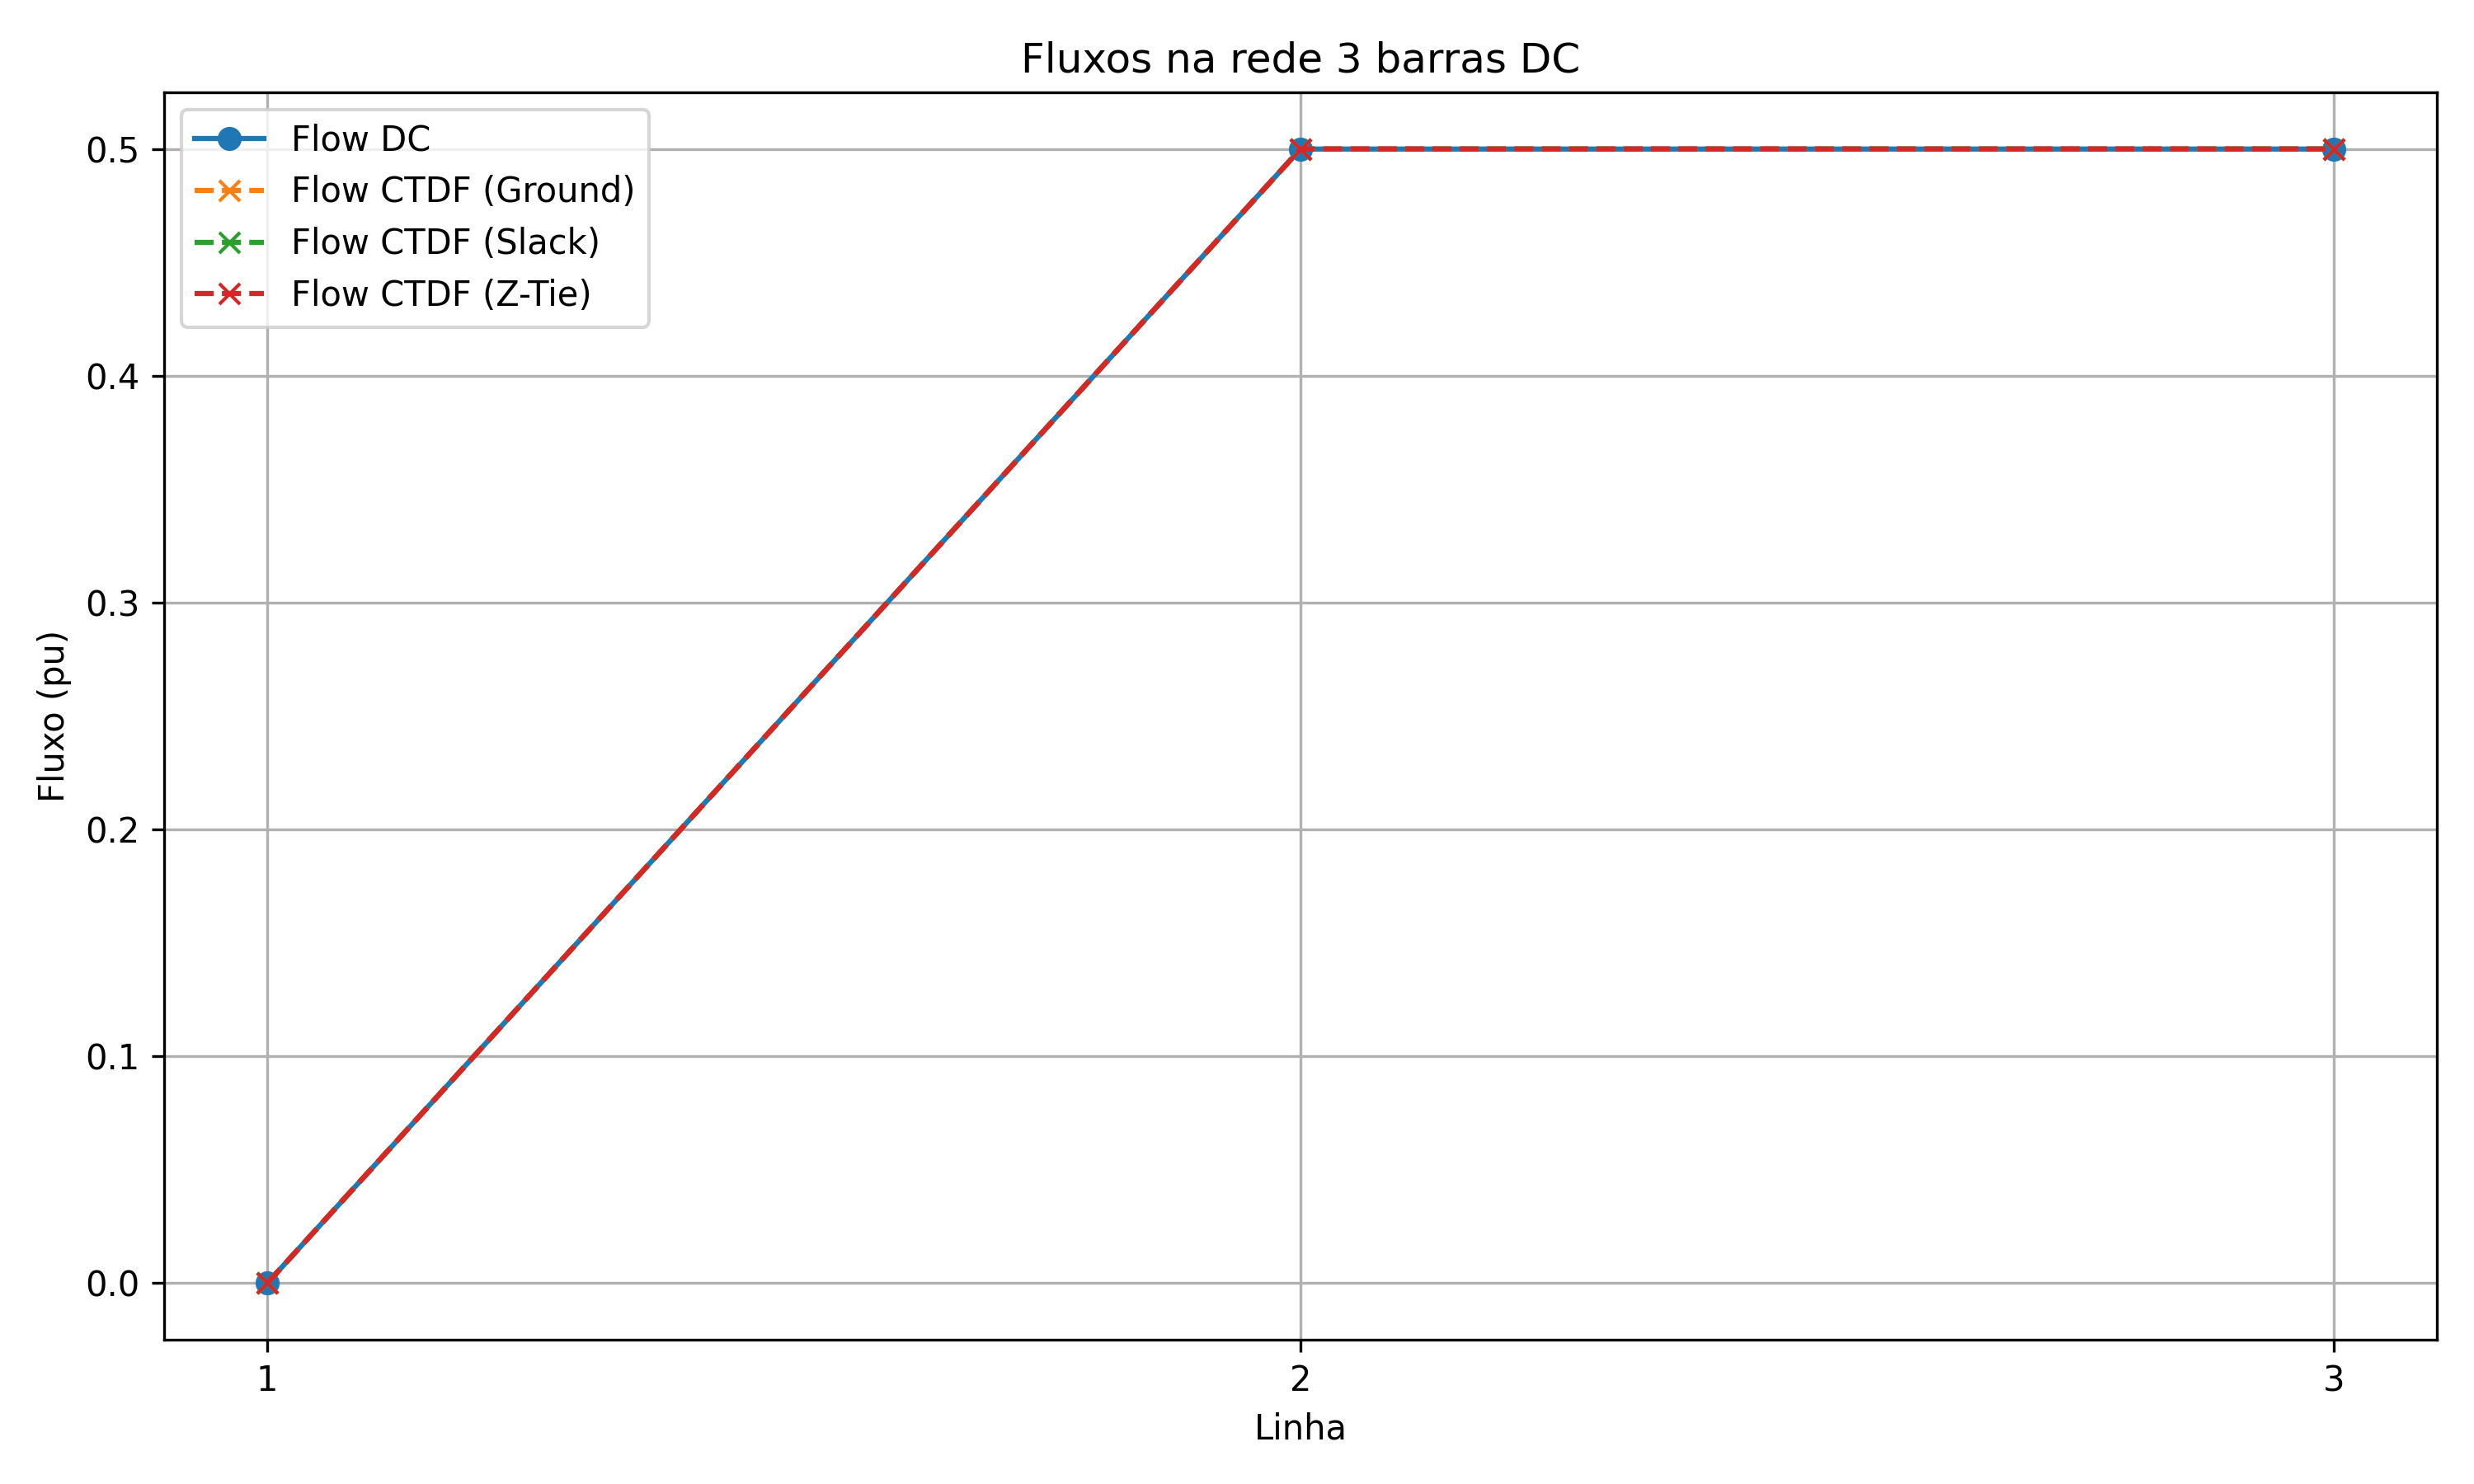
\includegraphics[width=1.0\linewidth]{../images/fluxos_3bus_DC.png}
\caption{Fluxos de potência cálculados por fatores de distribuição e fluxo DC}
\label{fig:fluxo_3bus_dc}
\end{figure}

Foram avaliadas as performances dos índices de distribuição com a rede em seu formato não linear, ou seja, agora com resistências nas linhas de transmissão. Para comparar com fluxos exatos AC e fluxos DC, consideramos dois casos:
\begin{enumerate}
  \item Aumento de 10\% de carga na barra 3;
  \item Aumento de 10\% de carga na barra 3 e 10\% de geração na barra 2;
\end{enumerate} 

As figuras \ref{fig:fluxo_3bus_carga10} e \ref{fig:fluxo_3bus_cargaeger10} correspondem aos dois casos, respectivamente.

\begin{figure}[H]
\centering
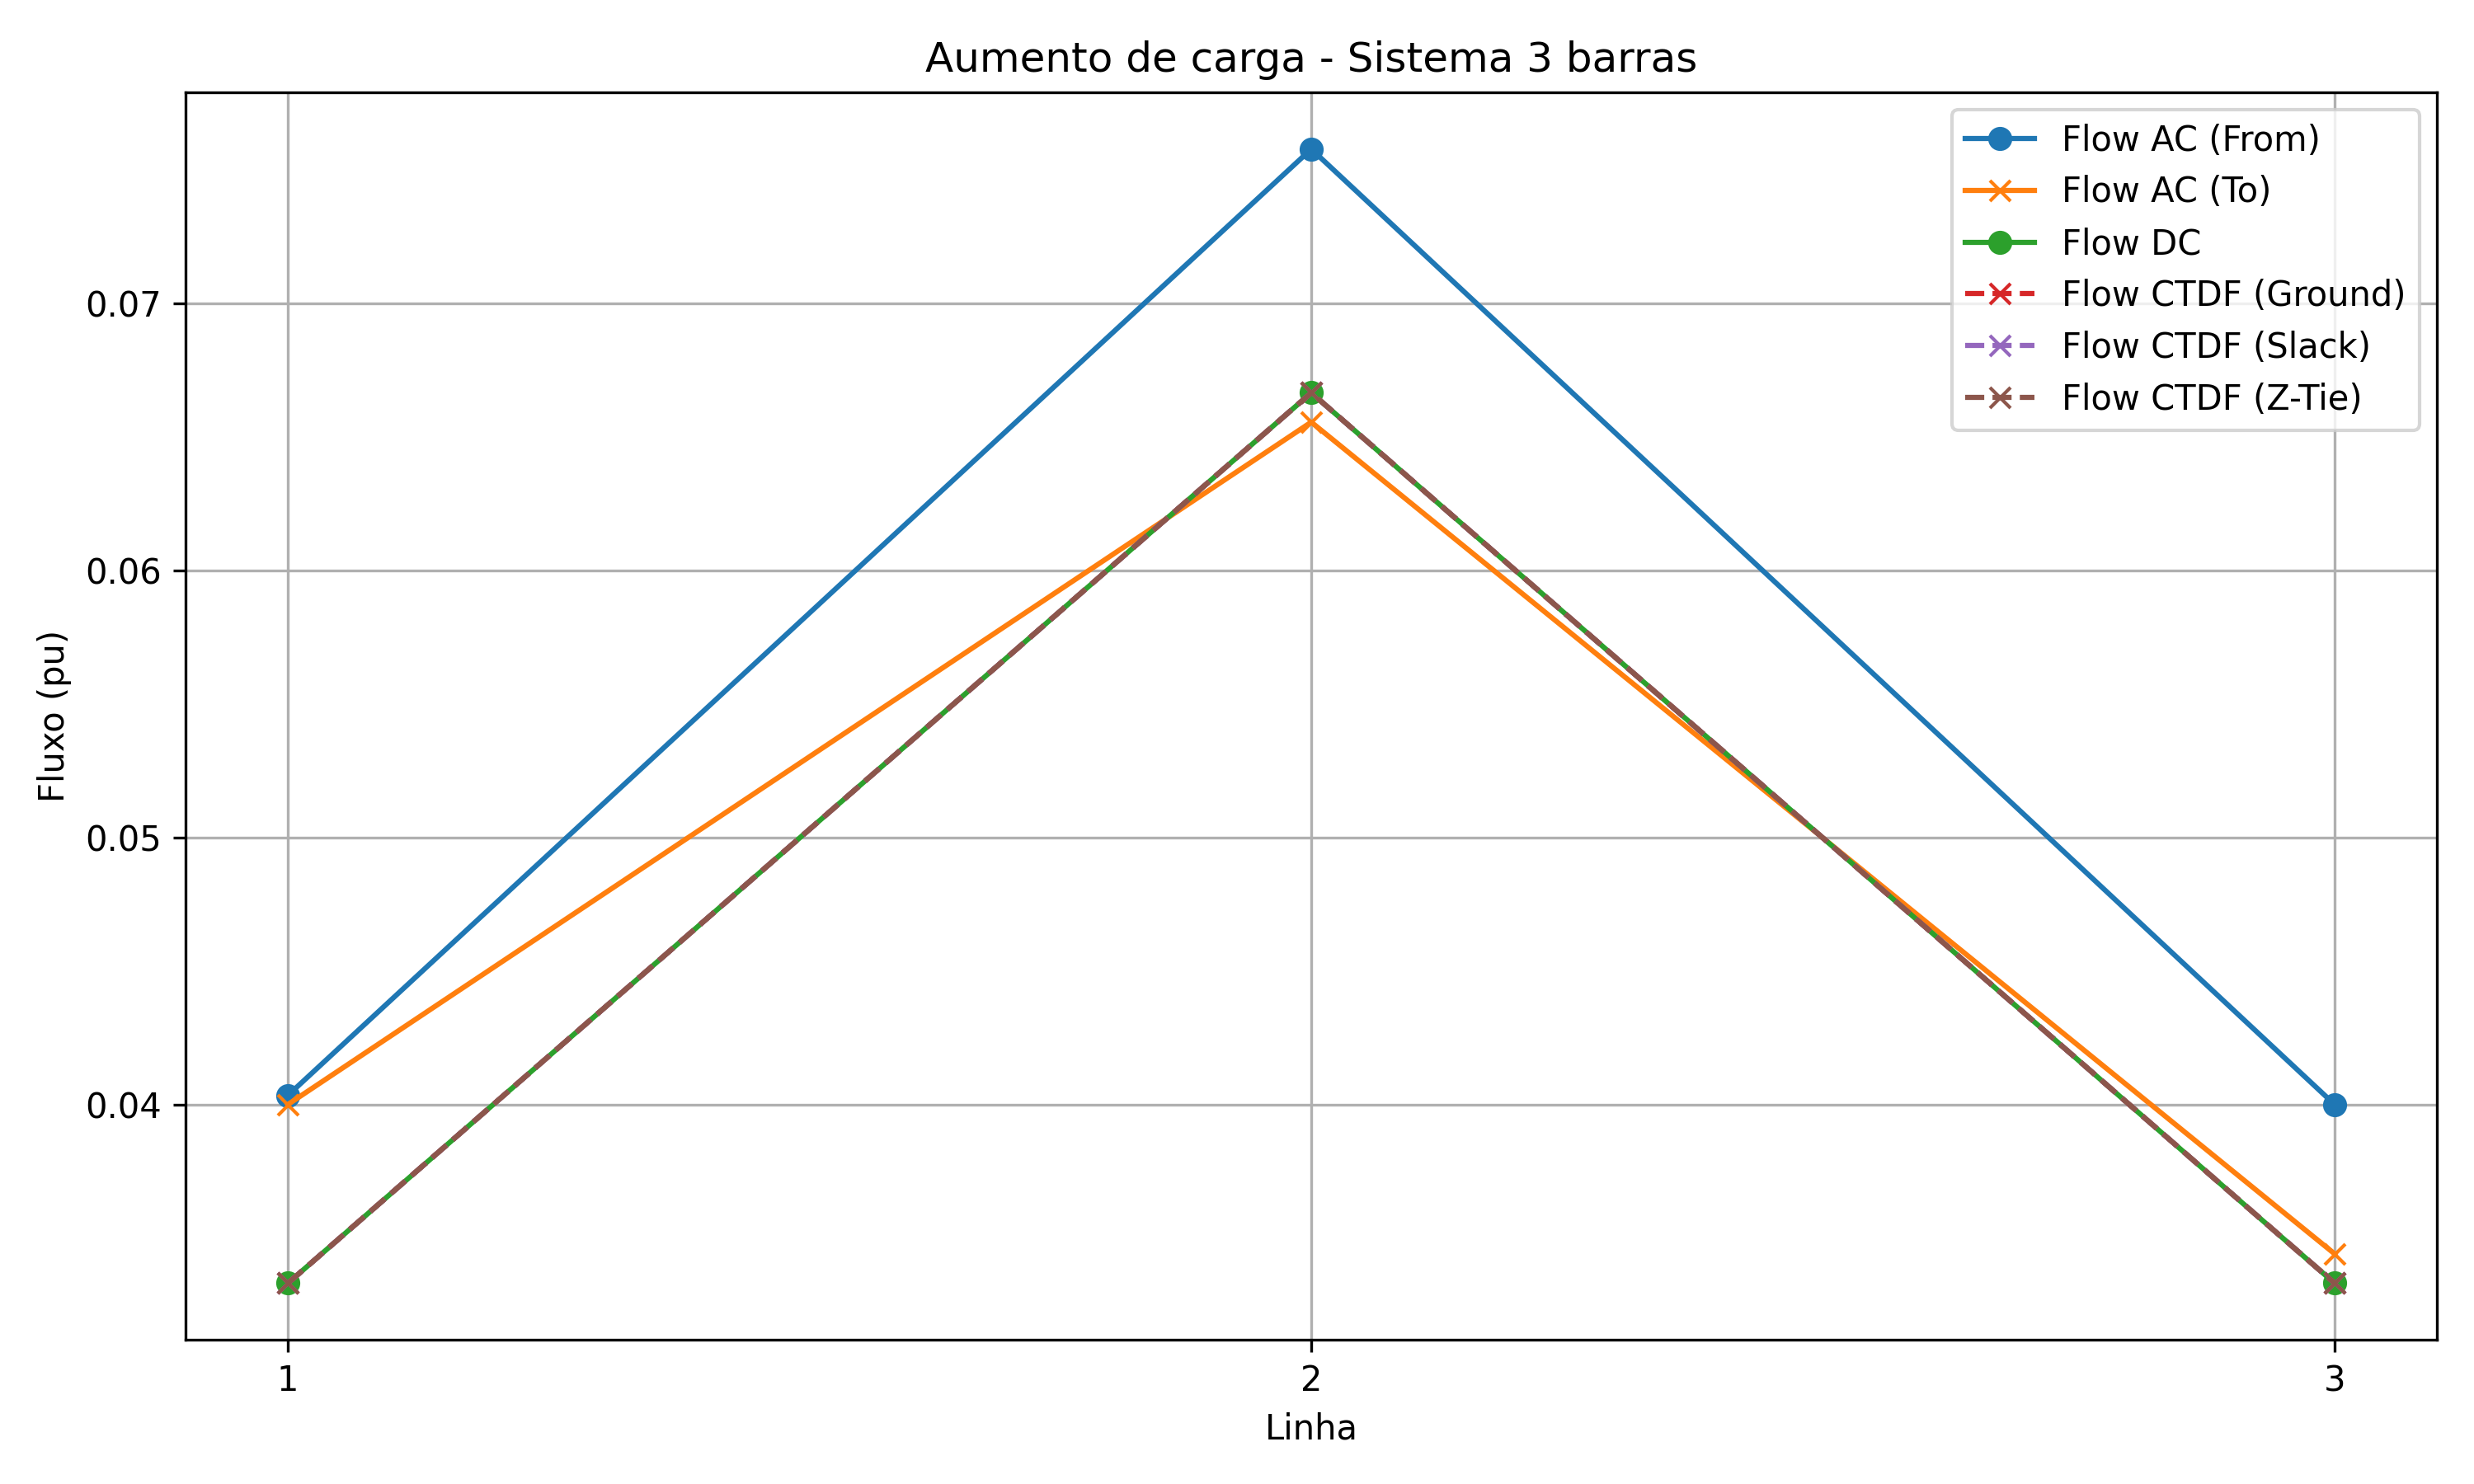
\includegraphics[width=1.0\linewidth]{../images/3bus_carga10.png}
\caption{Variação de fluxos com aumento de 10\% na barra $PQ$}
\label{fig:fluxo_3bus_carga10}
\end{figure}

\begin{figure}[H]
\centering
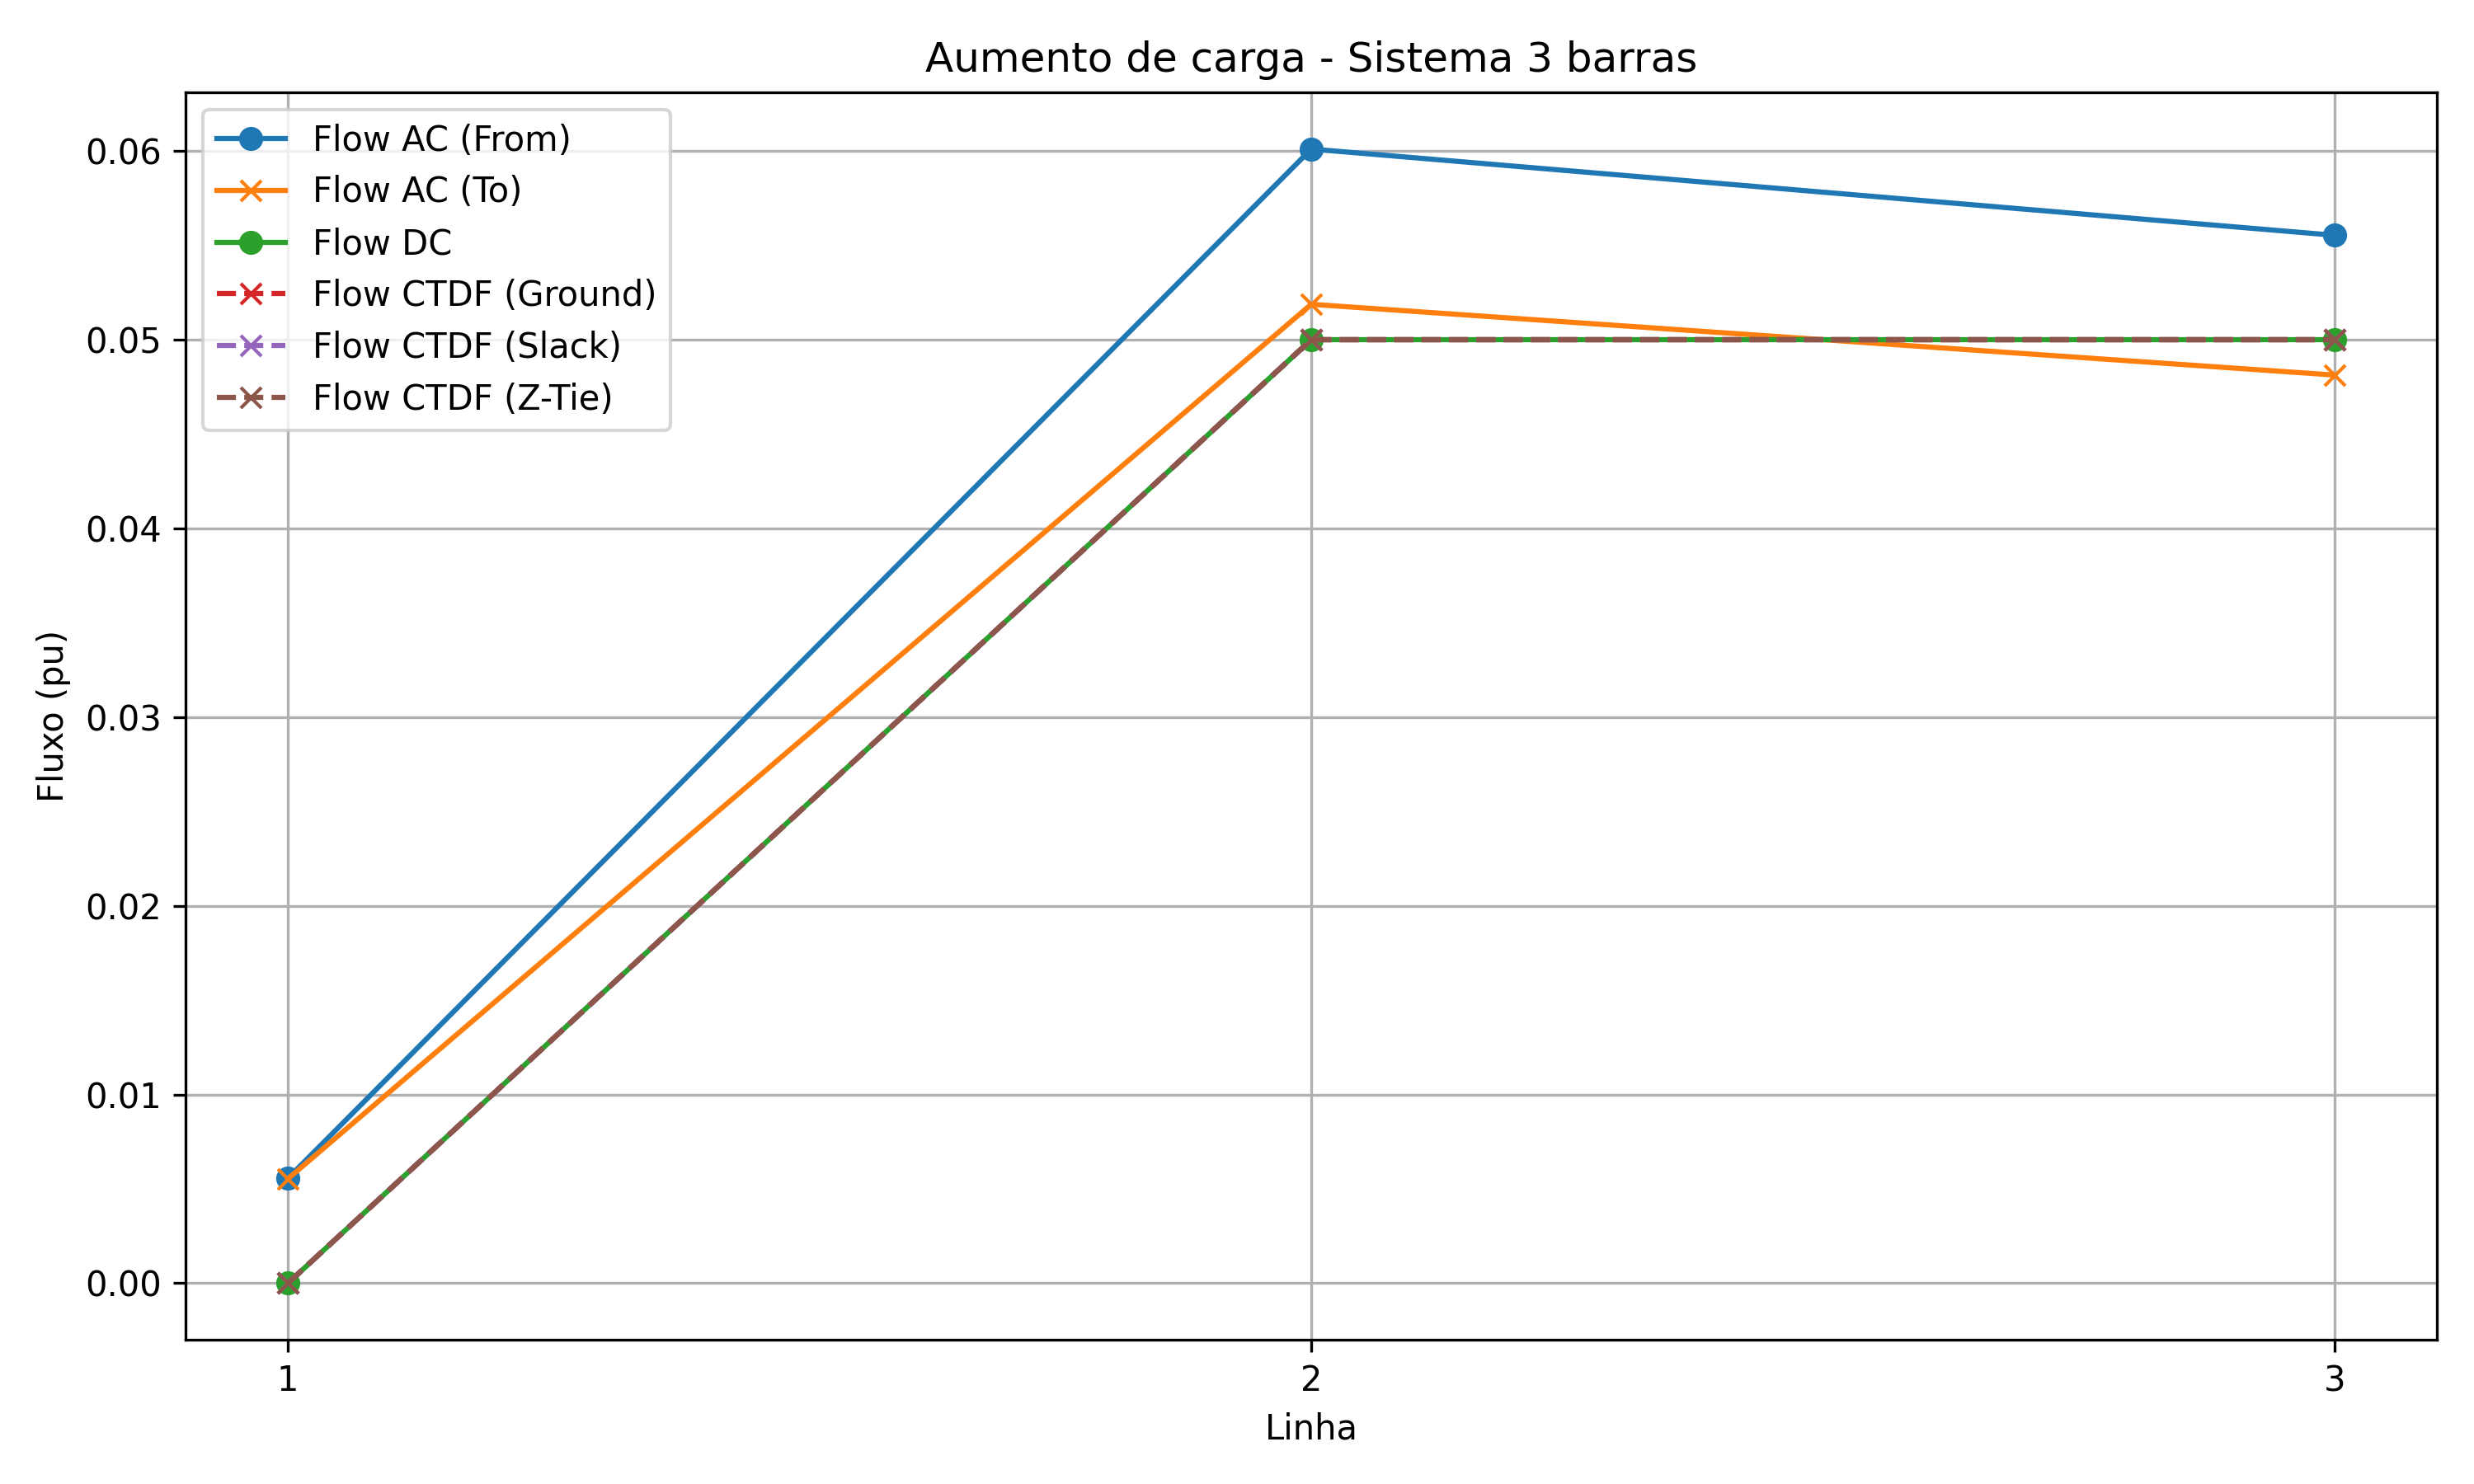
\includegraphics[width=1.0\linewidth]{../images/3_bus_cargaegeracao10.png}
\caption{Variação de fluxos com aumento de 10\% de carga na barra $PQ$ e 10\% de geração na barra $PV$}
\label{fig:fluxo_3bus_cargaeger10}
\end{figure}

Pode-se perceber que mesmo com a inclusão de resistências no sistema, as variações de fluxos obtidas através dos índices CTDFs foram idênticas às variações de fluxo obtidas através do fluxo DC.

De acordo com Sauer \cite{ref1}, a razão entre as admitâncias shunt e as reatâncias da linha podem impactar na performance dos índices, distintos dos fluxos DC. Para validar isso, foram adicionados shunts em todas as linhas com razão $r = b/x$ de 5\%, 20\% e 50\% e novamente a comparação entre os métodos foi feita em um caso de aumento de 10\% de carga na barra 3. foi calculado o erro médio dos desvios de fluxo em relação aos fluxos exatos AC, dados pelas equações \ref{eq:erro_from}, \ref{eq:erro_to} e \ref{eq:erro_medio}. Os resultados estão descritos na Tabela~\ref{tab:erro_3bus_bx}.

\begin{equation}
\text{Erro}_{\text{from}} = \frac{1}{n} \sum_{i=1}^{n} \left| \frac{\Delta F^{\text{método}}_i - \Delta F^{\text{AC, from}}_i}{\Delta F^{\text{AC, from}}_i} \right| \times 100\%
\label{eq:erro_from}
\end{equation}

\begin{equation}
\text{Erro}_{\text{to}} = \frac{1}{n} \sum_{i=1}^{n} \left| \frac{\Delta F^{\text{método}}_i - \Delta F^{\text{AC, to}}_i}{\Delta F^{\text{AC, to}}_i} \right| \times 100\%
\label{eq:erro_to}
\end{equation}

\begin{equation}
\text{Erro}_{\text{médio}} = \frac{1}{2} \left( \text{Erro}_{\text{from}} + \text{Erro}_{\text{to}} \right)
\label{eq:erro_medio}
\end{equation}

\begin{table}[!ht]
\centering
\caption{Erro percentual médio dos métodos para diferentes razões $r = b/x$ no sistema 3 barras}
\label{tab:erro_3bus_bx}
\begin{tabular}{l|ccc}
\hline
Método & $r=0.05$ & $r=0.20$ & $r=0.50$ \\
\hline
DC                & 12.01 & 13.48 & 13.31 \\
$CTDF_{ground}$   & 15.55 & 24.52 & 30.25 \\
$CTDF_{slack}$    & 10.97 & 10.28 & 6.90 \\
$CTDF_{ztie}$     & 16.26 & 28.71 & 37.26 \\
\hline
\end{tabular}
\end{table}

Pode-se perceber que, para este sistema, a formulação via método $CTDF_{slack}$ produziu resultados com menores erros médios nos 3 casos analisados.


\subsection{6 barras}
Para o sistema de 6 barras, foi aplicado um aumento de 10\% em todas as cargas e efetuado os mesmos cálculos de $\Delta P_{ij}$ para todos os métodos. Os erros médios estão descritos na tabela \ref{tab:erro_6bus}.

\begin{table}[!ht]
\centering
\caption{Erro percentual médio dos métodos para o sistema 3 barras}
\label{tab:erro_6bus}
\begin{tabular}{l|c}
\hline
Método            & Erro percentual médio (\%) \\
\hline
DC                & 59.69 \\
$CTDF_{ground}$   & 106.54 \\
$CTDF_{slack}$    & 52.39 \\
$CTDF_{ztie}$     & 85.46 \\
\hline
\end{tabular}
\end{table}

Os resultados mostram uma grande erro médio. Mas ainda assim, a formulação $CTDF_{slack}$, produziu erros inferiores à aproximação DC do sistema.




\section{Conclusões}
Neste trabalho, revisitou-se a formulação dos fatores de distribuição de corrente (CTDFs) para métodos lineares de fluxo de potência, conforme proposto por Sauer, e avaliou-se seu desempenho em sistemas teste de 3 e 6 barras. Foram implementados e comparados os métodos AC, DC e as diferentes variantes dos CTDFs (ground, slack e z-tie), considerando cenários com e sem elementos shunt, bem como diferentes políticas de despacho.

Os resultados confirmam que, em sistemas linearizados, os CTDFs reproduzem exatamente o fluxo DC, validando a equivalência teórica entre as abordagens. Para sistemas não lineares ou com a presença de elementos shunt, observou-se que o erro dos métodos lineares aumenta, mas ainda assim as aproximações são satisfatórias para aplicações de análise rápida, planejamento e estudos de sensibilidade. Destaca-se que a escolha da referência dos CTDFs (especialmente a slack) pode impactar significativamente a precisão dos resultados, sendo importante adequar a formulação ao contexto do sistema analisado.

Em síntese, os fatores de distribuição de corrente se mostraram ferramentas eficientes e versáteis para estimativa de fluxos em redes elétricas, proporcionando rapidez computacional e boa precisão em uma ampla gama de situações práticas.  Como trabalhos futuros, sugere-se a aplicação dos CTDFs em sistemas reais de maior porte, bem como a investigação de extensões para considerar perdas e elementos shunt de forma mais precisa.
Uma outra possível oportunidade de pesquisa é a utilização dos índices CTDFs para cálculo de fluxos de potência ativa e reativa nas linhas em problemas de otimização, podendo ser mais realista que um modelo DC, com equações lineares, e sem variáveis de ângulo e módulo de tensões nodais.
\section*{Agradecimentos}
Agradecemos ao professor João Alberto Passos Filho, por disponibilizar o material de suporte, e incentivar o desenvolvimento do artigo. 



% {\appendix[Proof of the Zonklar Equations]
% Use $\backslash${\tt{appendix}} if you have a single appendix:
% Do not use $\backslash${\tt{section}} anymore after $\backslash${\tt{appendix}}, only $\backslash${\tt{section*}}.
% If you have multiple appendixes use $\backslash${\tt{appendices}} then use $\backslash${\tt{section}} to start each appendix.
% You must declare a $\backslash${\tt{section}} before using any $\backslash${\tt{subsection}} or using $\backslash${\tt{label}} ($\backslash${\tt{appendices}} by itself
%  starts a section numbered zero.)}



%{\appendices
%\section*{Proof of the First Zonklar Equation}
%Appendix one text goes here.
% You can choose not to have a title for an appendix if you want by leaving the argument blank
%\section*{Proof of the Second Zonklar Equation}
%Appendix two text goes here.}



% \section{References Section}
% You can use a bibliography generated by BibTeX as a .bbl file.
%  BibTeX documentation can be easily obtained at:
%  http://mirror.ctan.org/biblio/bibtex/contrib/doc/
%  The IEEEtran BibTeX style support page is:
%  http://www.michaelshell.org/tex/ieeetran/bibtex/
 
%  % argument is your BibTeX string definitions and bibliography database(s)
% %\bibliography{IEEEabrv,../bib/paper}
% %
% \section{Simple References}
% You can manually copy in the resultant .bbl file and set second argument of $\backslash${\tt{begin}} to the number of references
%  (used to reserve space for the reference number labels box).

\begin{thebibliography}{1}
\bibliographystyle{IEEEtran}

\bibitem{ref1}
P. W. Sauer, ``On the formulation of power distribution factors for linear load flow methods,'' \textit{IEEE Trans. Power Appar. Syst.}, vol. PAS-100, no. 2, pp. 764--770, Feb. 1981. DOI: 10.1109/TPAS.1981.316422.


\end{thebibliography}


\newpage

\section{Biography Section}

\begin{IEEEbiography}[{\vspace{-1mm}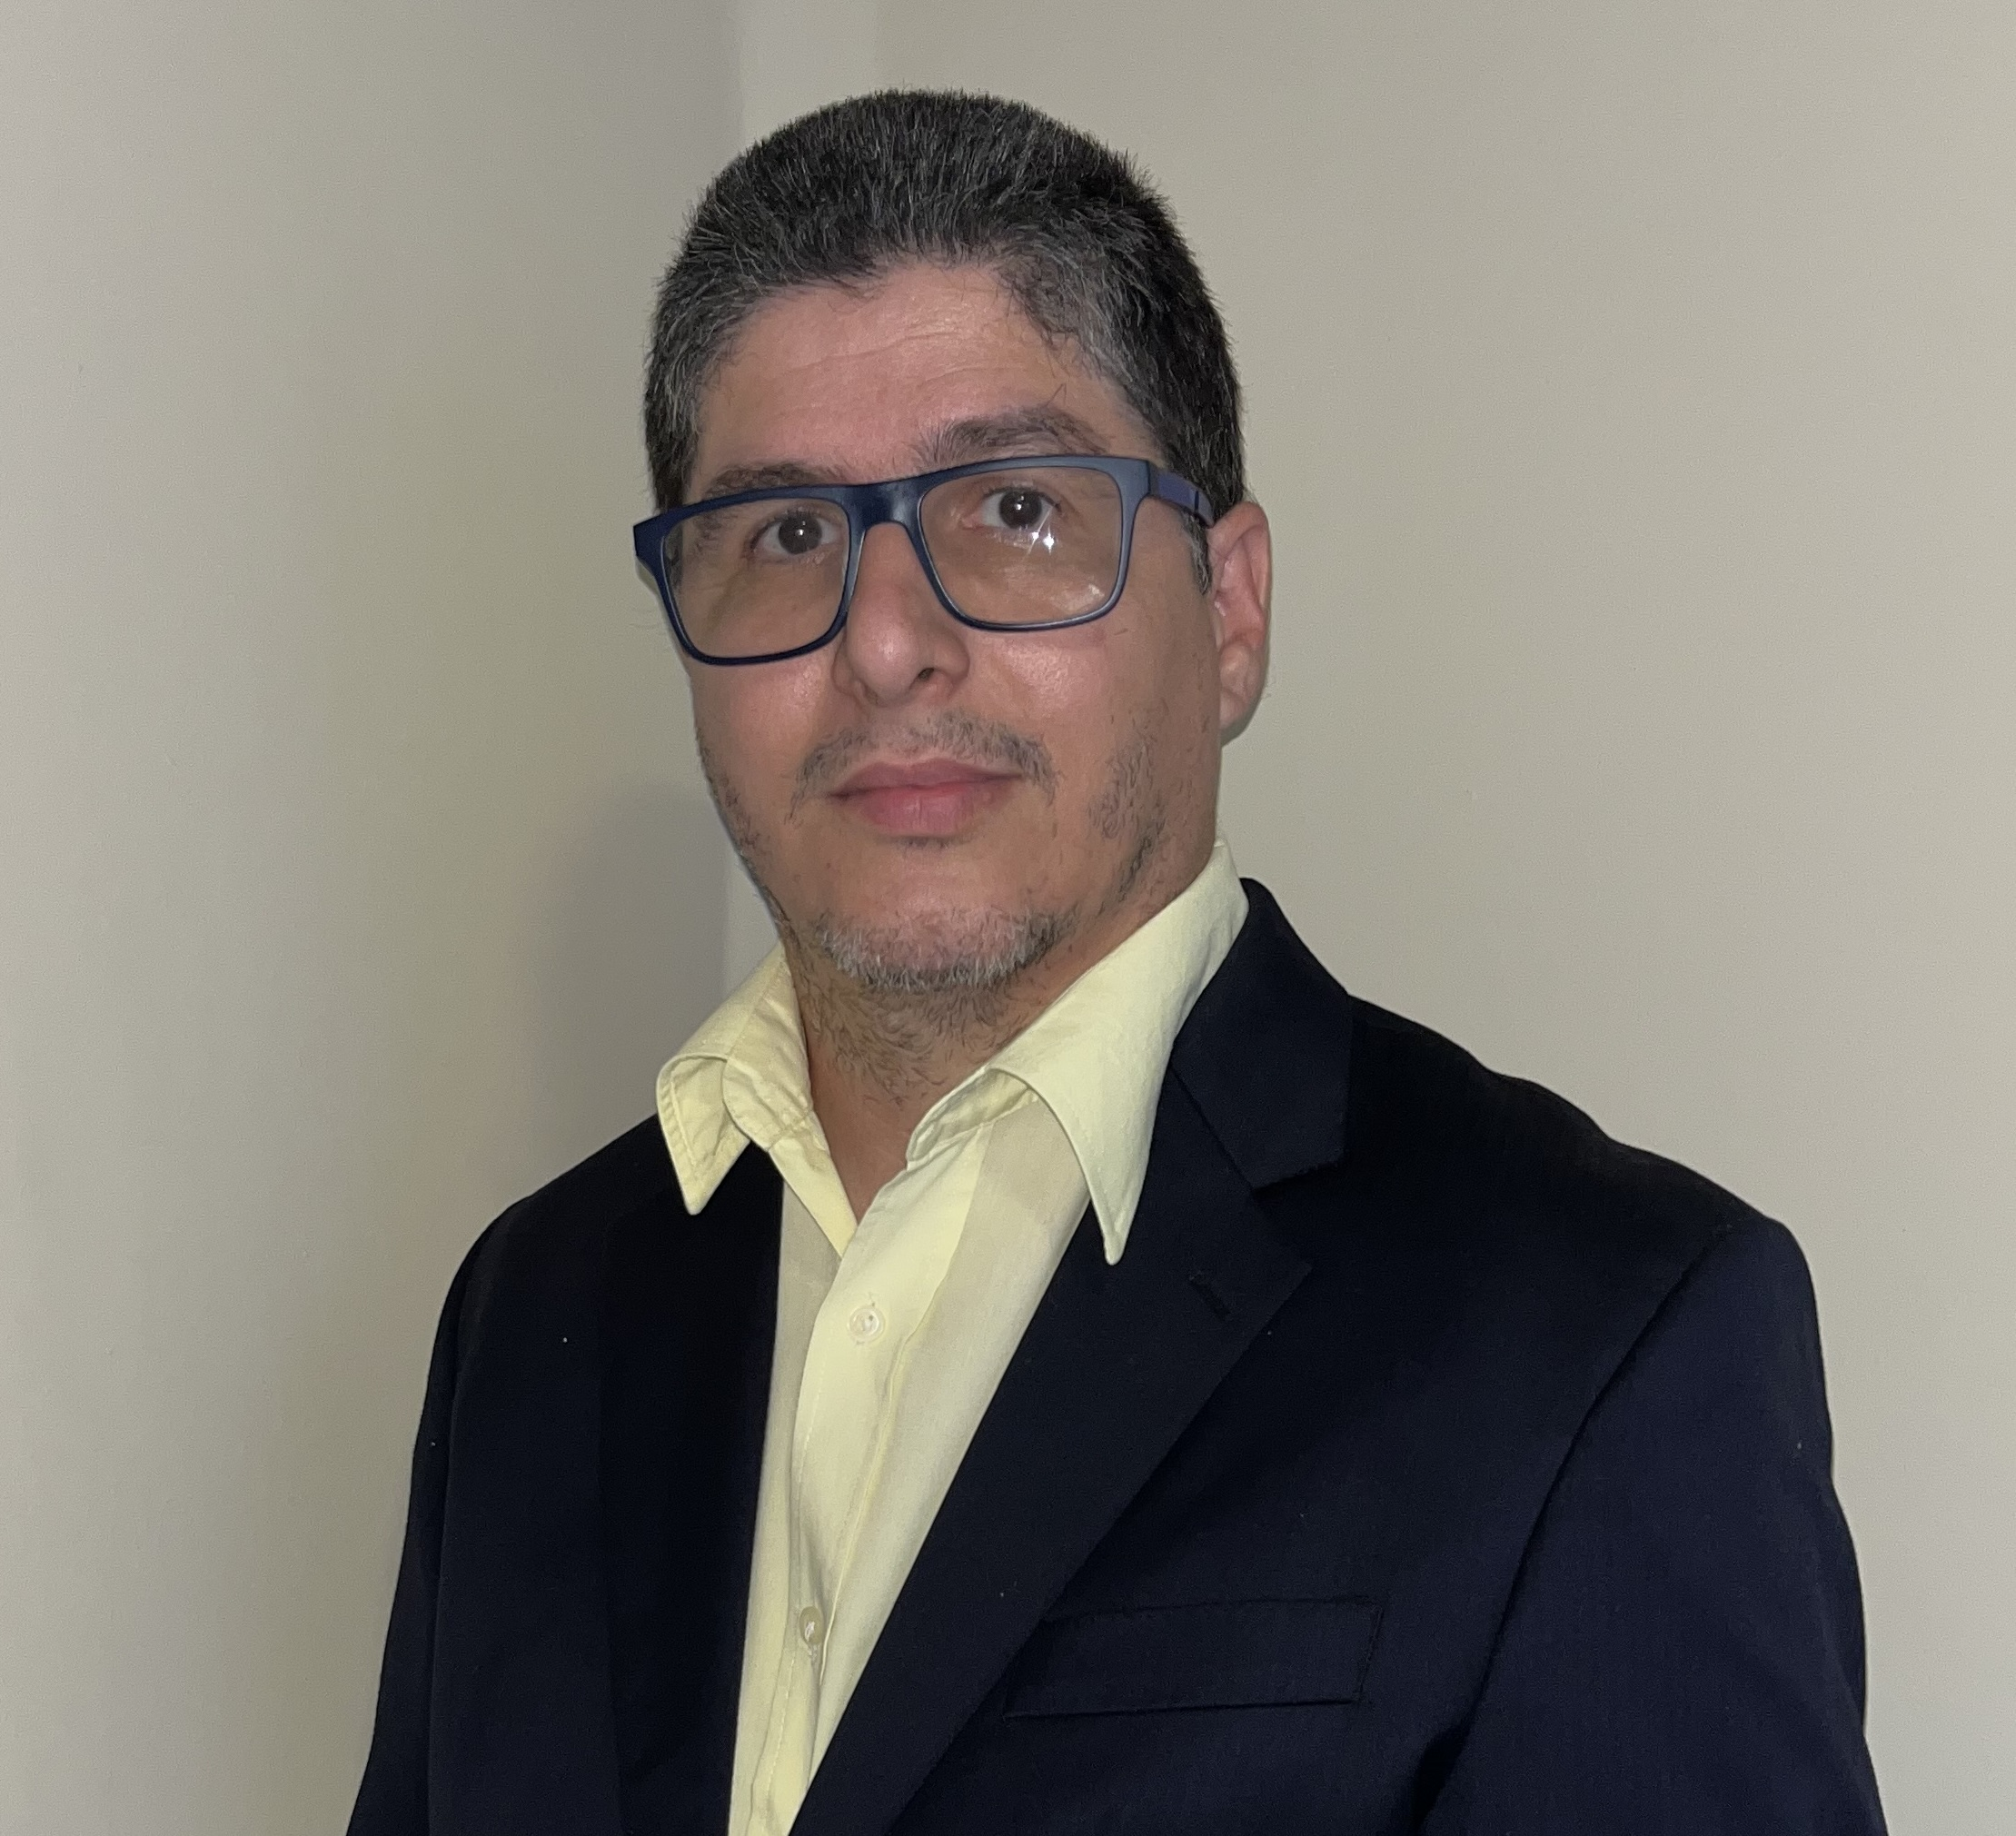
\includegraphics[width=1in,height=1.25in,clip,keepaspectratio]{../images/giovani_foto.jpg}}]{Giovani Santiago Junqueira}
Possui graduação em Engenharia Mecânica pela EESC-USP, pós-graduação em Engenharia de Manutenção pela UNITINS e MBA Executivo em Administração do Setor Elétrico pela FGV. Atua há mais de 23 anos em usinas hidrelétricas no setor elétrico brasileiro. Atualmente é aluno de mestrado em Engenharia Elétrica de Potência pela Universidade Federal de Juiz de Fora, com foco em métodos de otimização e confiabilidade de sistemas elétricos.
\end{IEEEbiography}

\begin{IEEEbiography}[{\vspace{-1mm}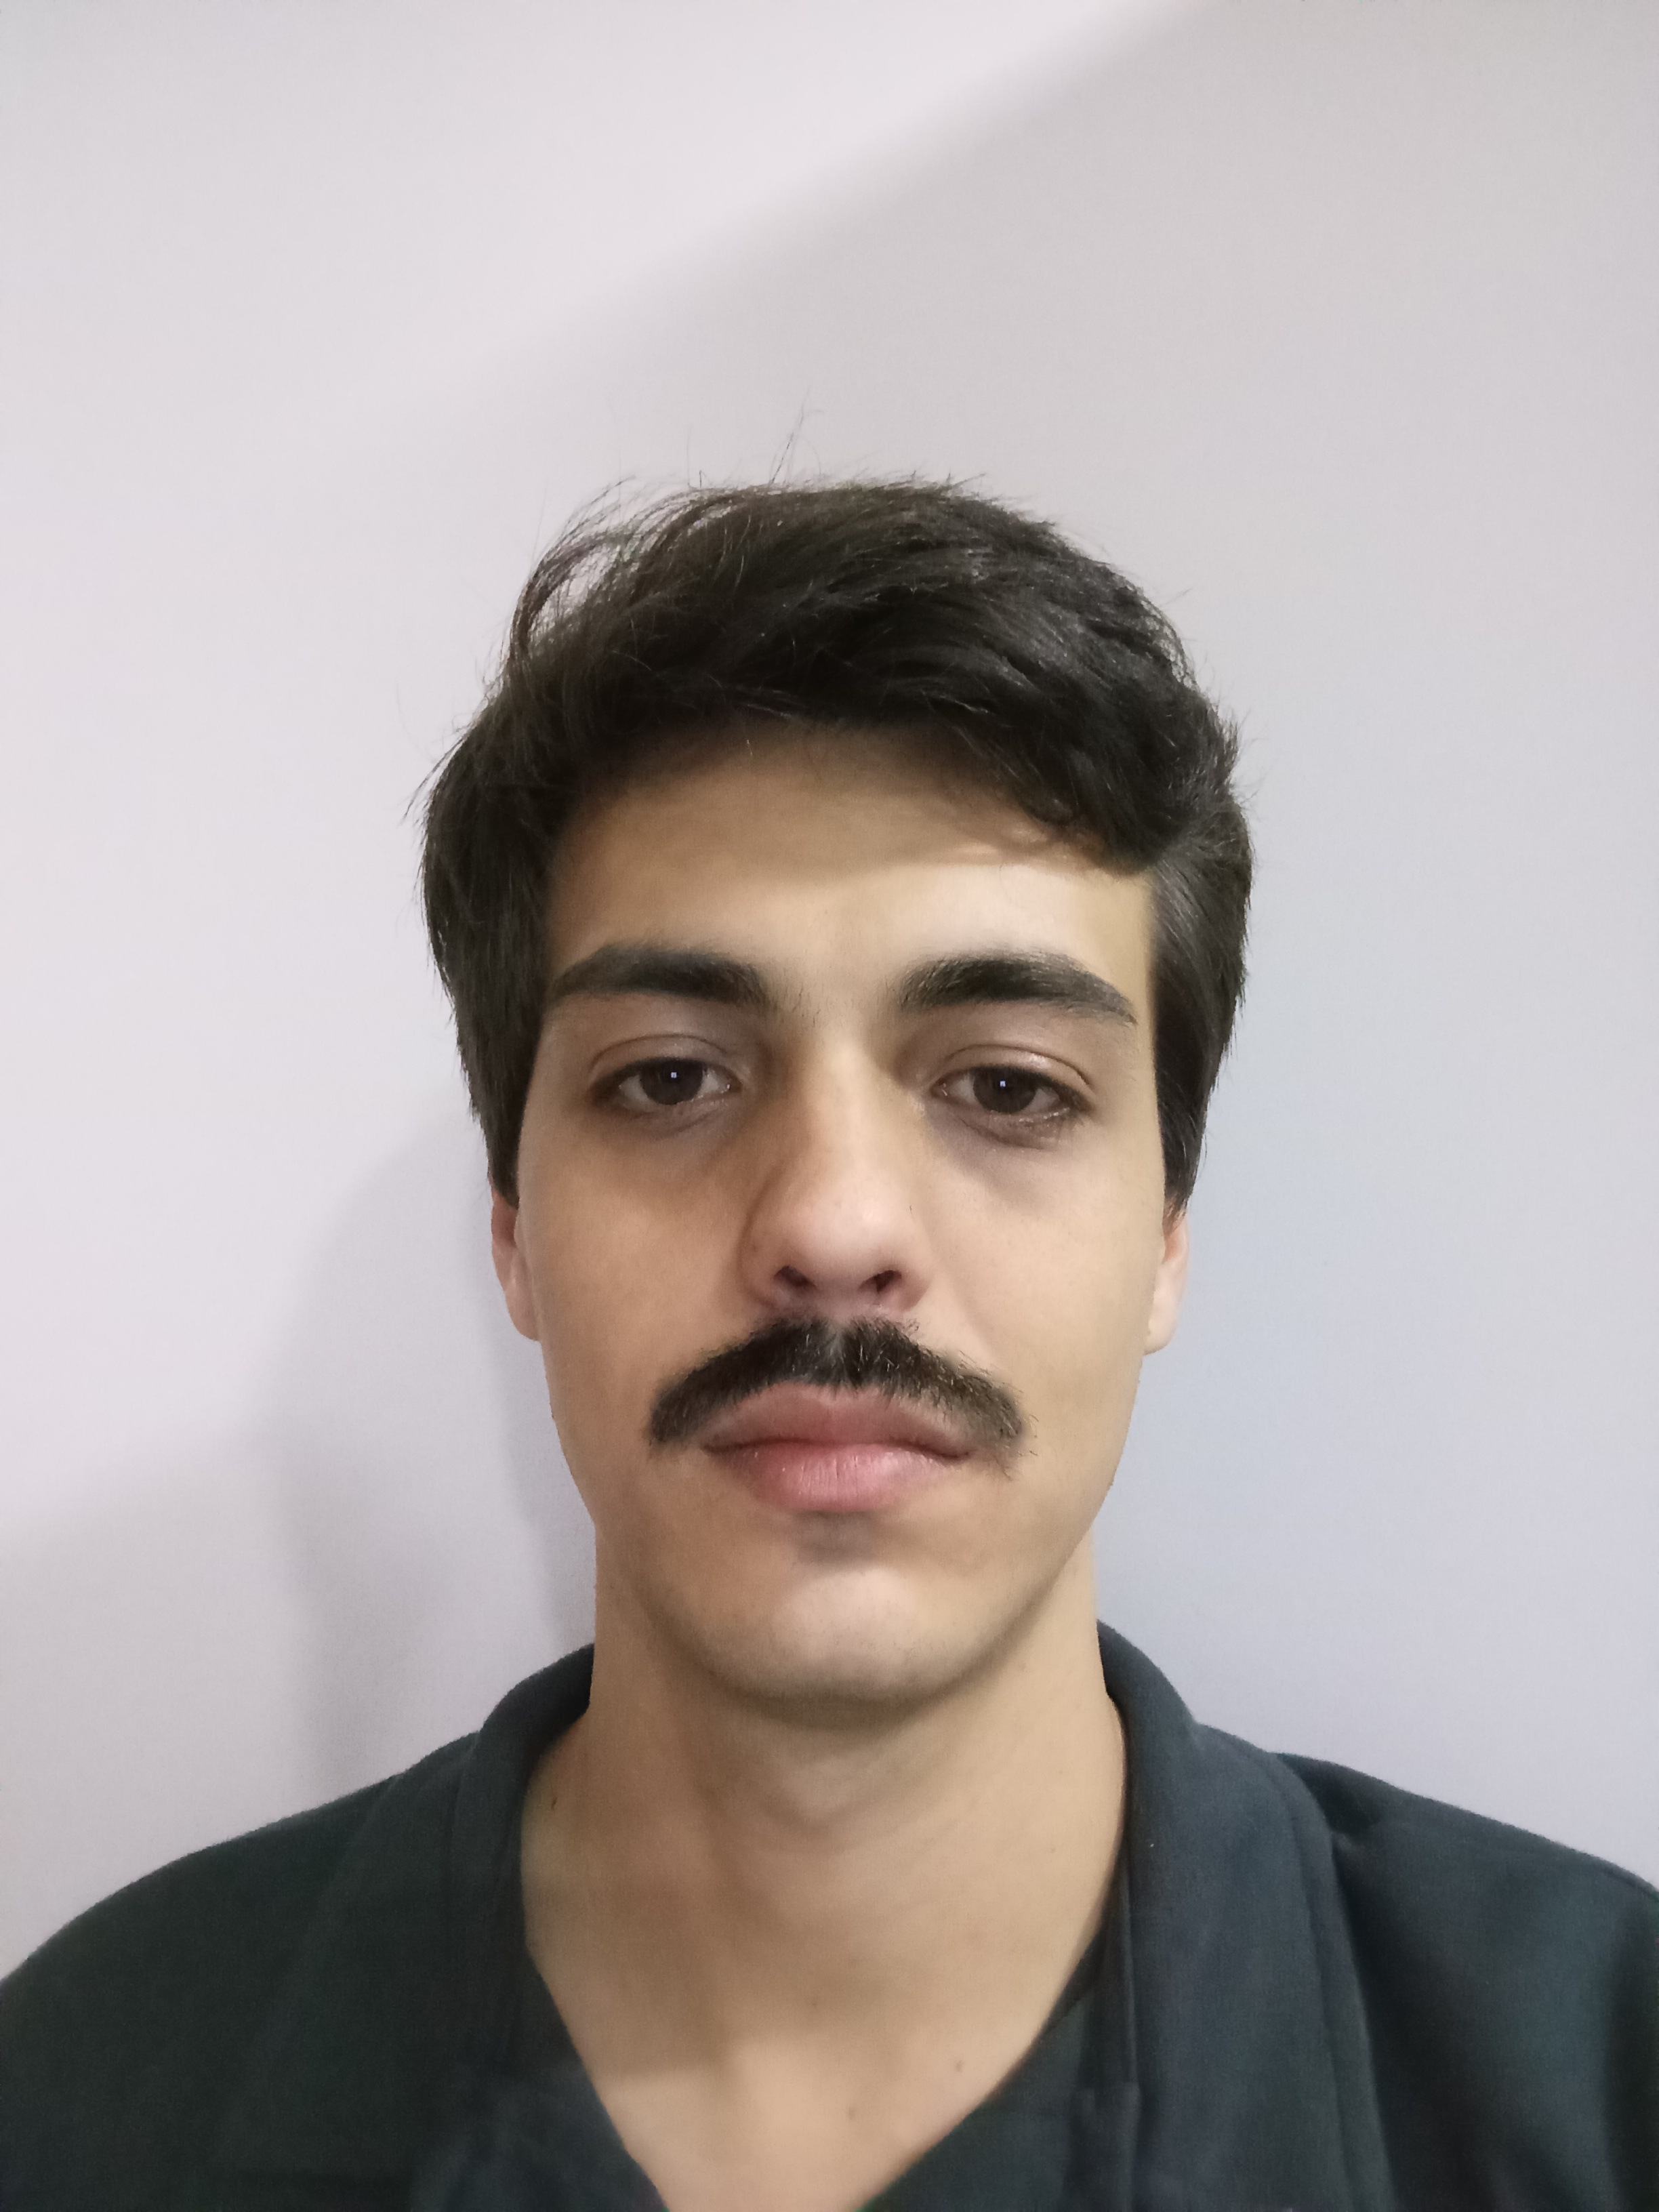
\includegraphics[width=1in,height=1.25in,clip,keepaspectratio]{../images/gabriel.jpg}}]{Gabriel Halfeld Limp de Carvalho}
É engenheiro eletricista formado pela Universidade Federal de Juiz de Fora (UFJF). Participou de projetos de extensão com foco em análise de fluxos de potência utilizando fractais de Newton. Atualmente, é mestrando em Engenharia Elétrica na UFJF, com atuação nas áreas de otimização de sistemas elétricos de potência como despacho econômico, mercado de energia e confiabilidade da operação.


\end{IEEEbiography}


\vfill
\clearpage
\appendix
\section{Dados e Imagens dos Sistemas de 3 e 6 Barras}

\subsection{Sistema de 3 Barras}
\begin{figure}[h!]
  \centering
  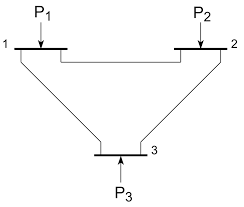
\includegraphics[width=0.4\textwidth]{../images/3_bus.png}
  \caption{Diagrama do Sistema de 3 Barras}
\end{figure}

\begin{table}[h!]
\centering
\caption{Dados das barras do Sistema de 3 Barras}
\label{tab:3bus_barras}
\begin{tabular}{c|c|c|c|c|c}
\hline
Barra & Tipo  & $V$ (pu) & $\theta$ (rad) & $P_{G}$ (pu) & $P_{C}$ (pu) \\
\hline
1 & Slack & 1.00 & 0.00 & --   & --   \\
2 & PV    & 1.00 & 0.00 & 0.5  & --   \\
3 & PQ    & 1.00 & 0.00 & --   & 1.0  \\
\hline
\end{tabular}
\end{table}

\vspace{1em}

\begin{table}[h!]
\centering
\caption{Dados das linhas do Sistema de 3 Barras}
\label{tab:3bus_linhas}
\begin{tabular}{c|c|c|c|c|c}
\hline
Linha & De & Para & $r$ (pu) & $x$ (pu) & $b/2$ (pu) \\
\hline
1 & 1 & 2 & 0.1 & 0.5 & 0 \\
2 & 1 & 3 & 0.1 & 0.5 & 0 \\
3 & 2 & 3 & 0.1 & 0.5 & 0 \\
\hline
\end{tabular}
\end{table}

\clearpage
\subsection{Sistema de 6 Barras}
\begin{figure}[h!]
  \centering
  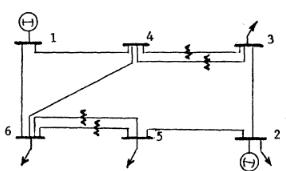
\includegraphics[width=0.4\textwidth]{../images/6bus.png}
  \caption{Diagrama do Sistema de 6 Barras}
\end{figure}

\begin{table}[h!]
\centering
\caption{Dados das barras do Sistema de 6 Barras de Sauer}
\label{tab:sauer6bus_barras}
\begin{tabular}{c|c|c|c|c|c|c}
\hline
Barra & Tipo  & $V$ (pu) & $\theta$ (rad) & $P_{G}$ (pu) & $P_{C}$ (pu) & $Q_{C}$ (pu) \\
\hline
1 & Slack & 1.05 & 0.00 & --    & --    & --    \\
2 & PV    & 1.10 & 0.00 & 0.50  & --    & --    \\
3 & PQ    & 1.00 & 0.00 & --    & 0.55  & 0.13  \\
4 & PQ    & 1.00 & 0.00 & --    & --    & --    \\
5 & PQ    & 1.00 & 0.00 & --    & 0.30  & 0.18  \\
6 & PQ    & 1.00 & 0.00 & --    & 0.50  & 0.05  \\
\hline
\end{tabular}
\end{table}

\begin{table}[h!]
\centering
\caption{Dados das linhas do Sistema de 6 Barras de Sauer}
\label{tab:sauer6bus_linhas}
\begin{tabular}{c|c|c|c|c|c|c|c}
\hline
Linha & De & Para & $r$ (pu) & $x$ (pu) & $b/2$ (pu) & Tap \\
\hline
1 & 1 & 4 & 0.080 & 0.370 & 0.00014 & 1.00 \\
2 & 1 & 6 & 0.123 & 0.518 & 0.00021 & 1.00 \\
3 & 2 & 3 & 0.723 & 1.050 & 0.00000 & 1.00 \\
4 & 2 & 5 & 0.282 & 0.640 & 0.00000 & 1.00 \\
5 & 4 & 6 & 0.097 & 0.407 & 0.00015 & 1.00 \\
6 & 4 & 3 & 0.000 & 0.266 & 0.00000 & 1.025 \\
7 & 4 & 3 & 0.000 & 0.266 & 0.00000 & 1.025 \\
8 & 6 & 5 & 0.000 & 0.428 & 0.00000 & 1.10 \\
9 & 6 & 5 & 0.000 & 1.000 & 0.00000 & 1.10 \\
\hline
\end{tabular}
\end{table}

\end{document}


